\documentclass[a4paper,10pt]{article}

% Wider pages.
\usepackage[a4paper]{geometry}

% Language.
\usepackage[english]{babel}

% Allows the use of \subtitle{...}.
\usepackage{titling}
\newcommand{\subtitle}[1]{%
  \posttitle{%
    \par\end{center}
    \begin{center}\large#1\end{center}
    \vskip0.5em}%
}

% Allows the use of \includegraphics{...}.
\usepackage{graphicx,subfigure}
\usepackage{amsmath}
% Allows the use of \url{...}.
\usepackage{url}

% Seperate paragraphs by an empty line and removes indentation.
\usepackage[parfill]{parskip}

\begin{document}

%%%%%%%%%%%%%%%%%%%%%%%%%%%%%%%%%%%%%%%%%%%%%%%%%%%%%%%%%%%%%%%%%%%%%%%%%%%%%%%
% TTITLEPAGE
%%%%%%%%%%%%%%%%%%%%%%%%%%%%%%%%%%%%%%%%%%%%%%%%%%%%%%%%%%%%%%%%%%%%%%%%%%%%%%%
\title{BioMAV: the package-inspecting robot}

\author{Robin Wellner and Roland Meertens}

\date{\today}

\maketitle

\section{Introduction}
BioMAV is a recurring project of the department of Artificial
Intelligence at the Radboud University in Nijmegen which stands for ``Biologically inspired Micro Air Vehicles''. In this report an overview will be given about what the project goals were this year. 

\subsection{Drone}
The robot used in the BioMAV is the Parrot AR.Drone 1.0. It is able to
communicate via USB and Wi-Fi. The drone has two cameras, one
ground-facing and one forward-facing. However, the driver software we
used was only able to access the image data from the forward-facing
camera.

\subsection{ROS}
ROS (for Robot Operating System) is an open-source framework for robot
controller software, especially intended for re-use of libraries
(called ``nodes'') between different projects and for different types of
robots. This allowed us to make use of existing solutions for blob
detection (used in section \ref{sec:corridorfollowing} and inter-node communication.

\subsection{Vision}
For vision the usage of CMVision turned out to be very handy for the detecting of blobs of colours. This was the reason that we used this for the detection of our goals. 
\section{Task}
\label{sec:task}
\subsection{Initial task}
\label{sec:initialtask}
The initial goals of this project were:
\begin{enumerate}
\item To establish a platform, based on the old BioMAV project, on which
      future BioMAV projects can build.
\item To let the drone perform a task autonomously. Which task that would be
      was to be determined.
\item To demonstrate the drone performing that task.
\end{enumerate}
\subsection{Final goal}
\label{sec:finalgoal}
Our final goal was to have the drone perform the packet-inspection task and
light-following task.

Initially we managed to create a fly-to-object behaviour. As this does not yet give way to a very advanced behaviour it was decided to add an implementation for a breadcrumbs finding navigation task. 

In this breadcrumbs navigation task the drone is able to locate a goal object by following other objects. 
Every time a temporary goal has been reached it will start searching for the next goal. 
\section{Method}
\subsection{Vision}


\subsection{Blob detection}
\subsubsection{Using cmvision}
We found a ROS package called cmvision that could find rectangular blobs of
roughly the same color in images, and could do that in real time. We used
it for every task. It was used both to find targets and recognise
corridors (see \ref{sec:pseudocode}).

cmvision comes with a tool, called colorgui, which allows one to calibrate the
range of values used to identify blobs. The dramatic influence of environment
lights on the colors meant that each time the environment changed, we had to
use the colorgui tool again to recalibrate the colors.

In our initial setup (with ROS Electric), cmvision did not specify correctly
which color each blob was. That meant we had to implement a few functions that
manually checked the colors of the camera pixel values. (See xxxx).


\subsection{Heat map}
\subsubsection{Idea}
At some point, it became clear that the blob detection was not consistent.
Small blobs were often found where none should be, and the blob corresponding
to the target fell away for a frame every so often. This confused the drone,
making navigation less than optimal.

We came with the idea of a heat map, which
would only activate after blobs appeared consistently on a certain position.
At the same time, a single missed frame wouldn't mean that the drone had lost
its target.
\subsubsection{How it works}\label{subsec:howheatmapworks}
The heat map is basically a matrix, each cell corresponding to a square of
pixels from the drone camera. Every blob detected would then increase the
values in the heat map inside that blob. Each time step, the matrix is
multiplied by a constant $c_{{cooldown}}$, where
$0 < c_{{cooldown}} < 1$, reducing the overall
activation.

Only if the maximal value in the matrix is more than a certain constant,
the drone considers doing anything based on the heat map that time step.
Otherwise, it will turn around slowly, looking for the target.

If the sum of all values in the matrix is more than another constant,
that means a large portion of the camera's field of vision is taken up
by the target, which means we're close to it. That means the drone has
found the target, and as such can continue to its next target.

In any case, each column in the matrix is summed, such that we have an
array of values. Each of these values is the total activation in a specific
column of the heat map. A high activation at a certain position means it is
likely that the target is in that position, and that means the drone should
fly in that direction. To figure out the ``centre of gravity'' of the
activation, we calculate the weighted average of the indexes of the columns,
with the array of values as weights. The result can be normalised, giving us
the direction the drone should fly.
\subsubsection{Implementation}
We used NumPy to deal with the matrix calculations.

The implementation has several constants that were abstracted from in the
previous section.

The multiplication constant $c_{{cooldown}}$ was taken to be
$0.5$. In our experience, larger values caused "after images" to persist
longer than needed, and smaller values reduced the positive effects of
the heat map too much, making jitters and missing blobs too strong.

The "downsize factor" by which the matrix was scaled down from the
drone camera was $4$, meaning that each cell in the heat map represented $16$
pixels. This was chosen because a smaller downsize factor would make the
algorithm that activated the heat map too slow, and with a downsize factor of
$4$, the resolution preserved was still sufficient for subtle steering
decisions.

The activation added for each blob depends on the blob area $A$. This was
another way to reduce the effect of jitters. The formula
that worked best for us was
\begin{align*}
 activation &=50 + \frac{\sqrt{A}}{10}
\end{align*}


The threshold that decided whether the drone has seen \emph{anything}
interesting was set to $16$, fairly arbitrarily.

The threshold for deciding the target has been found and the drone was
finished or needed to find another target, is strongly dependent on the
real life size of the target. Our targets were about $\frac{1}{4} m^2$
and the constant that worked best was $30 000$.

\subsubsection{...}

\subsection{Control}

\subsection{Flying towards objects\label{flytowards}}
\begin{verbatim}
direction = XvalueOfAverageOfActivation
turnTowards(direction)
flyForward
\end{verbatim}
XvalueOfAverageOfActivation is determined by using this formula: (as explained in \ref{subsec:howheatmapworks})
\[\texttt{XvalueOfAverageOfActivation} = 0.5 - \frac{Avg}{i_{max}}\]
\[Avg = weighted-average([0, ..., i_{max} - 1], weights=weights)\]
\[weights_i = \sum_{j=0}^{j_{max}-1} H_{ij} \]
\[H = \textrm{(heat map matrix, $i_{max}$ columns, $j_{max}$ rows)}\]

\subsection{Package inspection\label{sec:packageinspection}}
\begin{verbatim}
if SumActivation > threshold
        currentTarget = getNewTarget(currentTarget)
    else
        startLanding
\end{verbatim}
The sum of activation if determined by using this formula: (as explained in \ref{subsec:howheatmapworks})
\[\texttt{SumActivation} = \sum_{i=0}^{i_{max}-1} \sum_{j=0}^{j_{max}-1} H_{ij}\]
\[H = \textrm{(heat map matrix, $i_{max}$ columns, $j_{max}$ rows)}\]

\section{Results}

\subsection{Github}
The source code to the ROSMAV project (as well as this report) are accessible
on Github. This is because it made working with multiple team members
reasonably convenient. Additionally, it makes ROSMAV easily accessible to
others, as they can simply clone or fork the repository from Github.
\subsection{Use case}


%%%%%%%%%%%%%%%%%%%%%%%%%%%%%%%%%%%%%%%%%%%%%%%%%%%%%%%%%%%%%%%%%%%%%%%%%%%%%%%
% INTRODUCTION
%%%%%%%%%%%%%%%%%%%%%%%%%%%%%%%%%%%%%%%%%%%%%%%%%%%%%%%%%%%%%%%%%%%%%%%%%%%%%%%
\section{Introduction}
%%%%%%%%%%%%%%%%%%%%%%%%%%%%%%%%%%%%%%%%%%%%%%%%%%%%%%%%%%%%%%%%%%%%%%%%%%%%%%%
\section{Background}
\label{sec:background}
\subsection{IMAV}
IMAV is a series of conferences and competitions with as main objective
``to provide an effective and established forum for dissemination and
demonstration of original and recent advances in MAV technology.''\cite{imav}
MAV stands for Micro Air Vehicles and IMAV stands for International
Micro Air Vehicles.

\subsection{BioMAV}
The previous and first BioMAV project started in 2010. It was the entry
of Radboud University Artificial Intelligence department. BioMAV was a large
success and obtained the third price in the IMAV 2011 pylon challenge.

\subsection{Biological inspiration}
This project's biological inspirations are mostly related to vision. The
corridor-following task described in section \ref{sec:corridorfollowing} was inspired by how flying insects such as moths
follow the light of the moon for navigation. The packet inspection task described in section \ref{sec:packageinspection}
evolved from animals hunting their prey.
\begin{figure}[h!]
	\caption{A picture of a drone.}
	\centering
	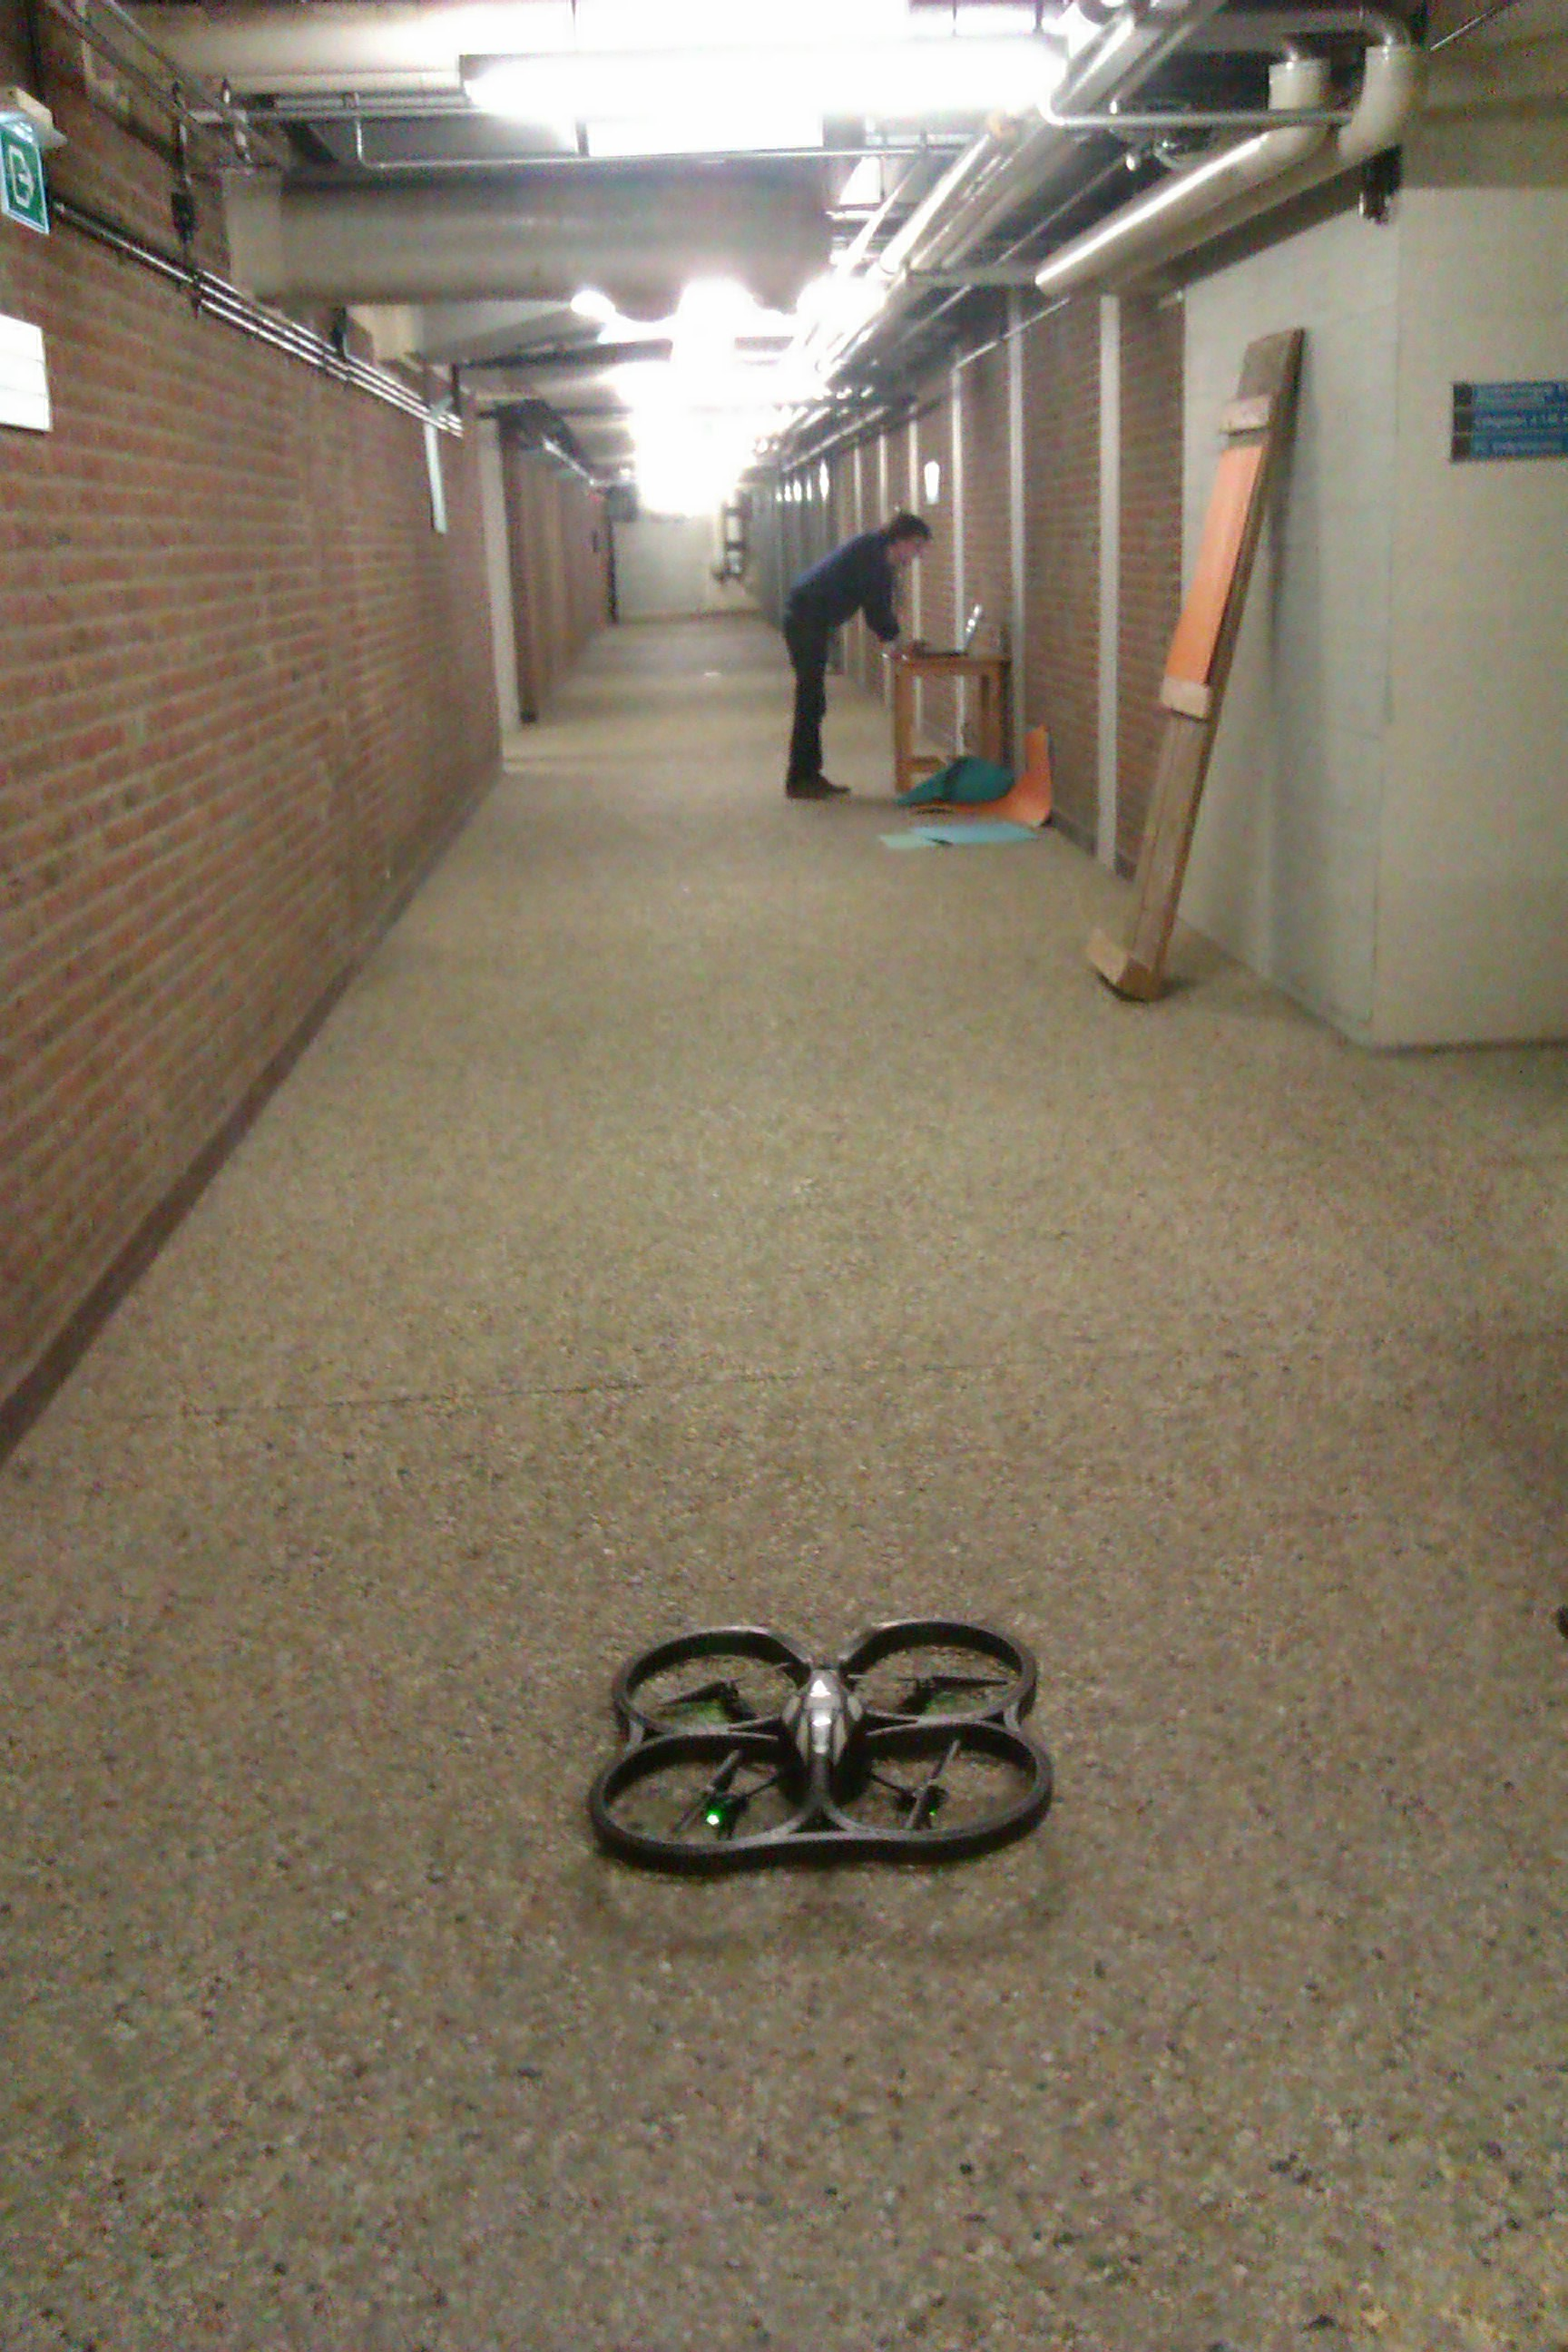
\includegraphics[width=0.5\textwidth]{images/boringHallway}
\end{figure}

In this section several of the implemented algorithms are discussed. Every subsection starts with the code in pseudocode and ends with an explanation of the algorithm. 

\begin{figure}[h!]
	\caption{Robin with a target in the left image, on the right is the activation}
	\centering
	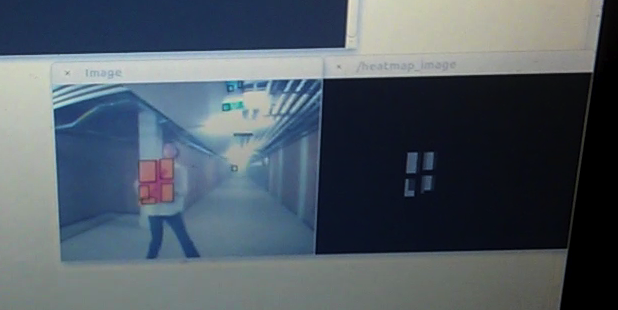
\includegraphics[width=0.5\textwidth]{images/robinPresentActivation}
	\label{fig:robinPresentActivation}
\end{figure}

\begin{figure}[h!]
	\caption{A picture of a drone.}
	\centering
	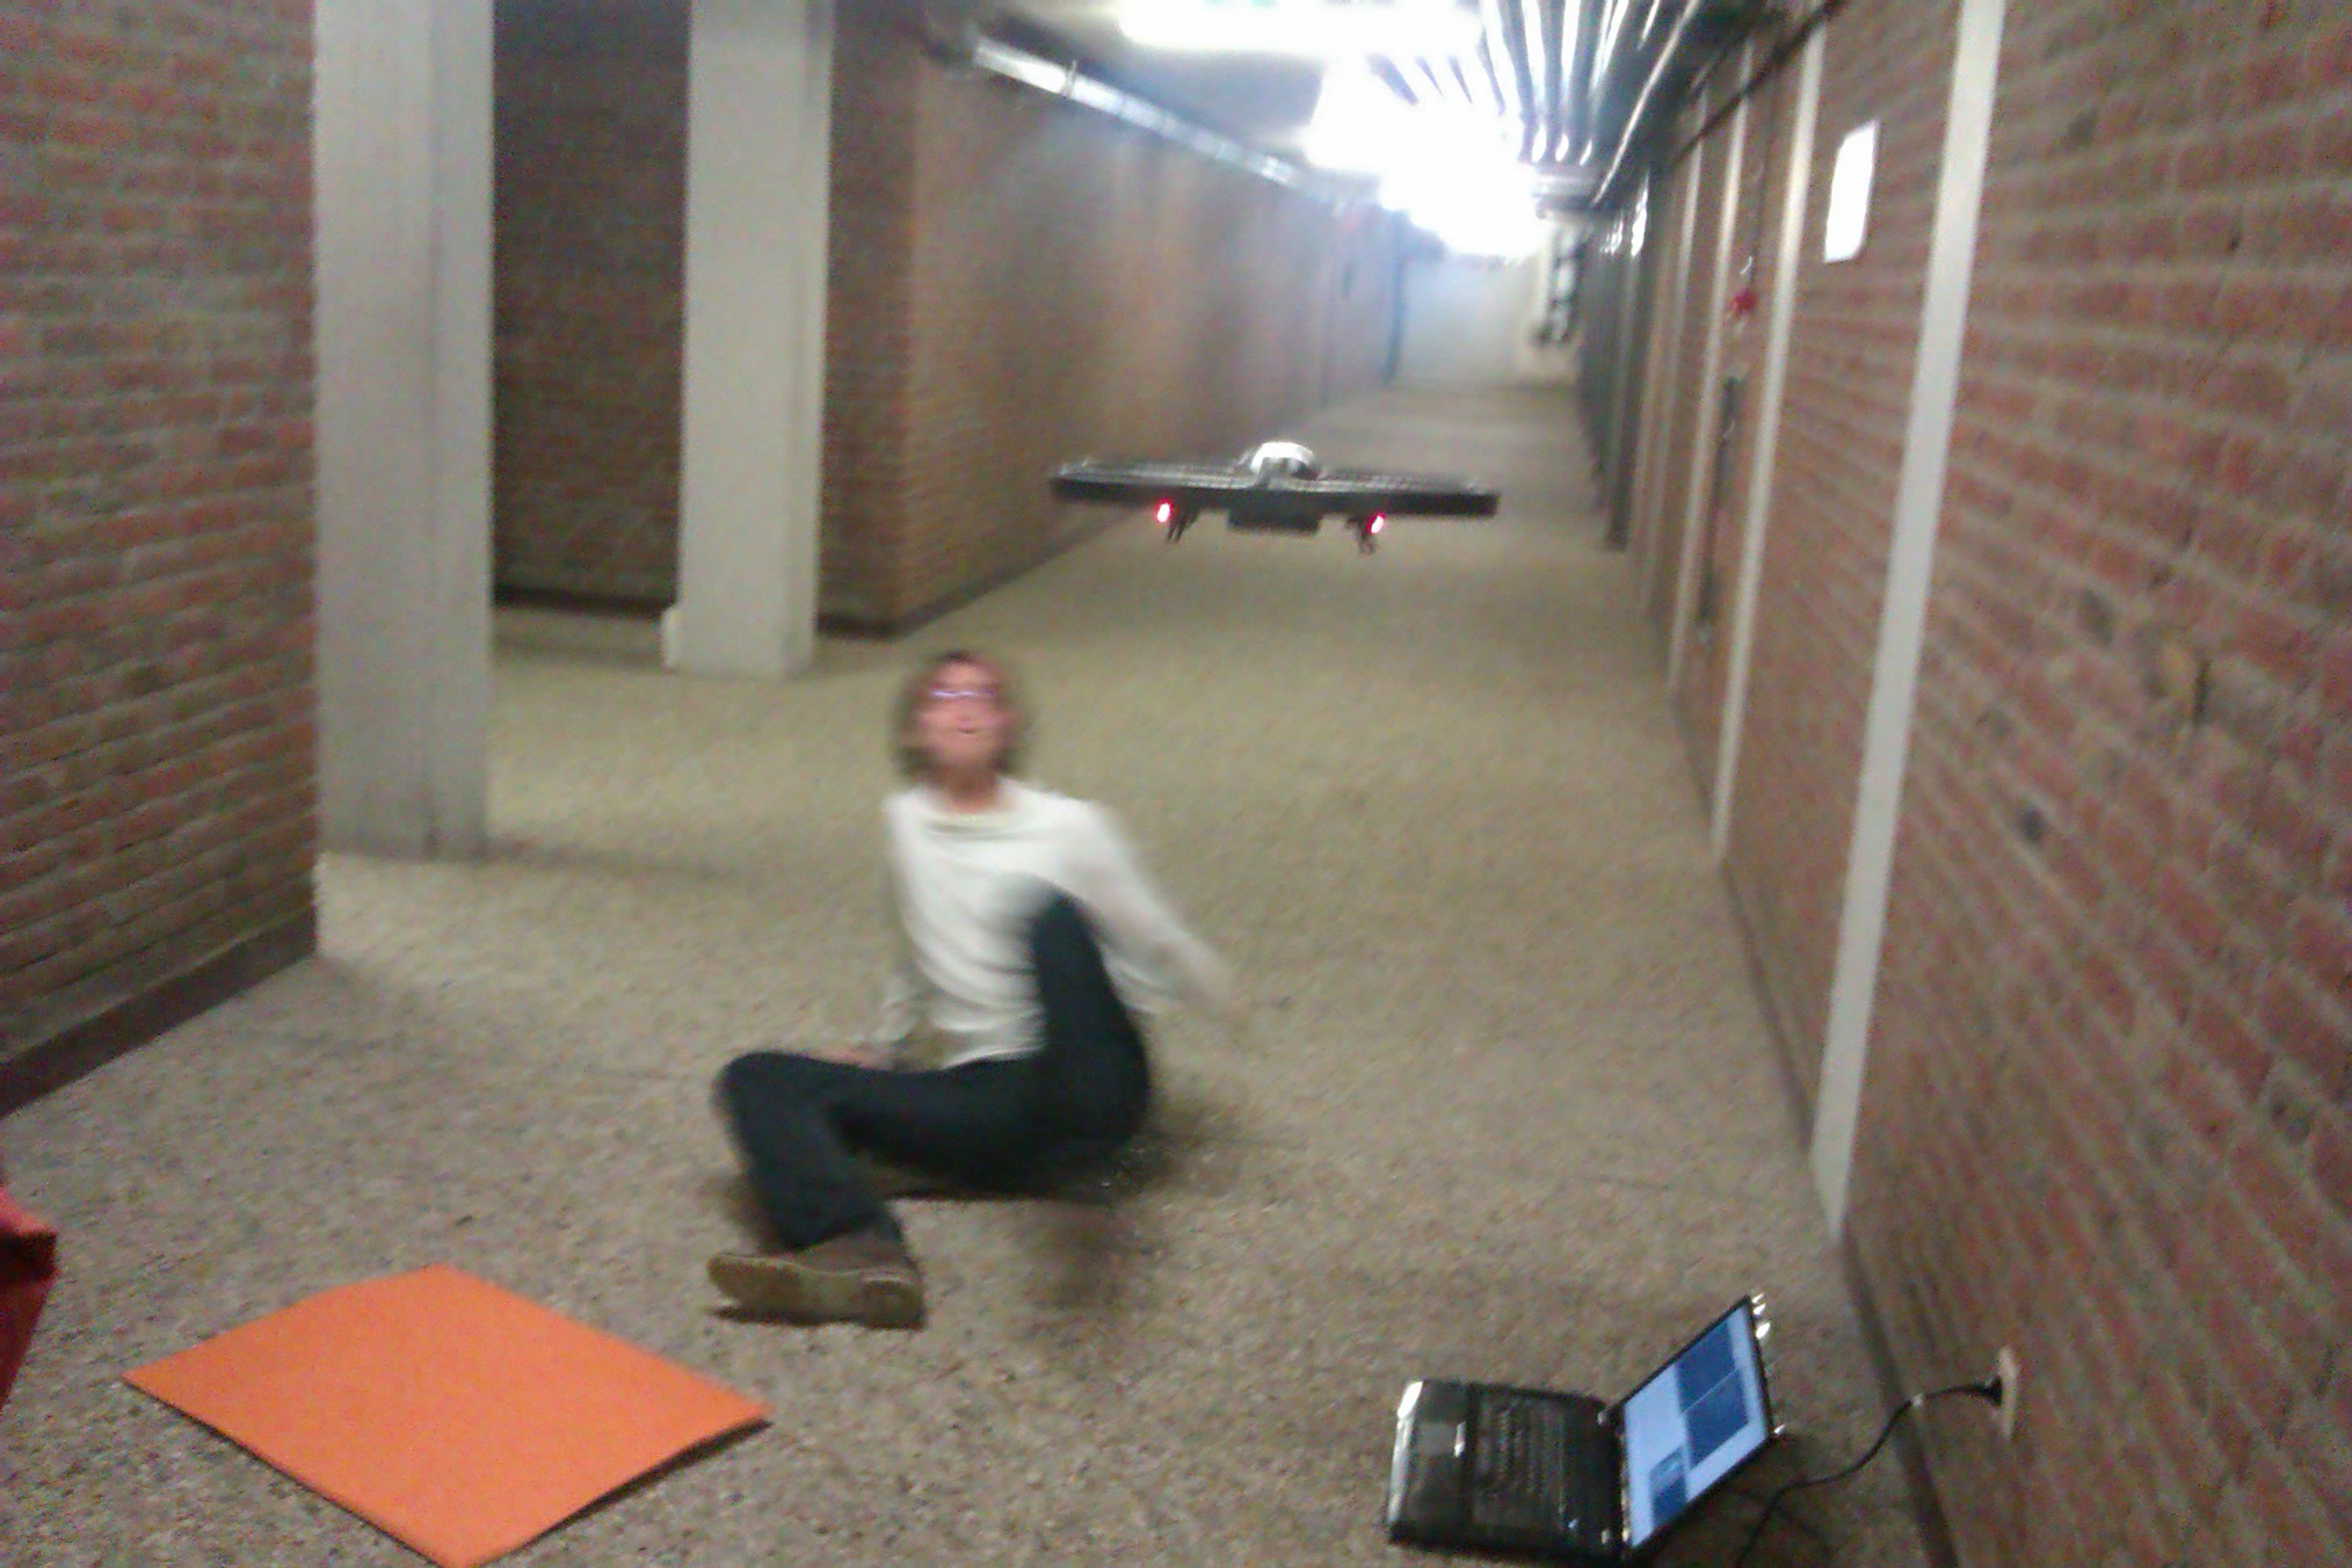
\includegraphics[width=0.5\textwidth]{images/droneAttack}
\end{figure}

%%%%%%%%%%%%%%%%%%%%%%%%%%%%%%%%%%%%%%%%%%%%%%%%%%%%%%%%%%%%%%%%%%%%%%%%%%%%%%%
% TUTORIAL
%%%%%%%%%%%%%%%%%%%%%%%%%%%%%%%%%%%%%%%%%%%%%%%%%%%%%%%%%%%%%%%%%%%%%%%%%%%%%%%
\section{Tutorial}
\subsection{Installation}
To install ROSMAV, follow the following steps:
\begin{enumerate}
\item Install Ubuntu (we used Ubuntu 10.10).

\item Install ROS (we used Electric) by following this guide: \\
      http://www.ros.org/wiki/electric/Installation/Ubuntu

\item Make sure that you performed the ``Environment setup'' step during installation.

\item Download our repository from
      https://github.com/dutchcheesehead/ROSMAV

\item Navigate to ROSMAV.

\item Run \textbf{./install.sh}.
\item Close your terminal window.
\end{enumerate}

\subsection{Starting ROSMAV}
To start our software, run the following commands all in different terminal windows:
\begin{enumerate}
\item \textbf{roscore} \\ This starts roscore.
\item \textbf{rosrun ardrone\_brown ardrone\_driver} \\ This starts the driver for the AR-Drone.
\item \textbf{roslaunch cmvision blobs.launch} \\ This starts the blob detection process.
\item \textbf{drone\_teleop.py} \\ This is needed to let the drone take off and land.
\item \textbf{rosrun image\_view image\_view image:=/heatmap\_image} \\ This
      allows you to see the heat map activation for the ``inspect presents''
      task, and thus see through the eyes of the drone.
\item \textbf{rosrun ROSMAV inspectPresents.py} \textit{or} \\
      \textbf{rosrun ROSMAV followLights.py} \\
      This actually starts the task. 
\end{enumerate}
\subsection{Adding different colors to inspect}
Suppose you want to add a different color to inspect.
\begin{enumerate}
\item Run \textbf{roscore}
\item In another terminal window, start the AR-Drone driver: \textbf{rosrun ardrone\_brown ardrone\_driver}
\item Start the ColorGUI: \textbf{rosrun cmvision colorgui image:=/ardrone/image\_raw} \\
      You will see a window with the camera images from the AR-Drone.
\item Resize the window so you can see the text fields.
\item Keep the object you want to inspect in the view of the drone.
\item Click on the image of that object in the ColorGUI on a few different places.
\item Move both the object and the drone a bit around and click some more, to account for changes in lighting.
\item Repeat until you are confident it recognizes the object correctly in different circumstances.
\item If you made a mistake, close the ColorGUI and go back to step 3.
\item If it recognizes the object correctly, open ``cmvision/colors.txt''. Add both the color and the threshold. For the color, you can copy the last color and change the first bit into what the ColorGUI said, and change the name of the color. For the threshold, paste the threshold after the last threshold.
\item Edit ``inspectPresents.py''. You might need to add a function like ``isRed'' if it's not already in there. Then modify the ``nextTarget'' dictionary to the sequence you want to inspect the presents.
\end{enumerate}

\begin{figure}[h!]
	\caption{A picture of a drone.}
	\centering
	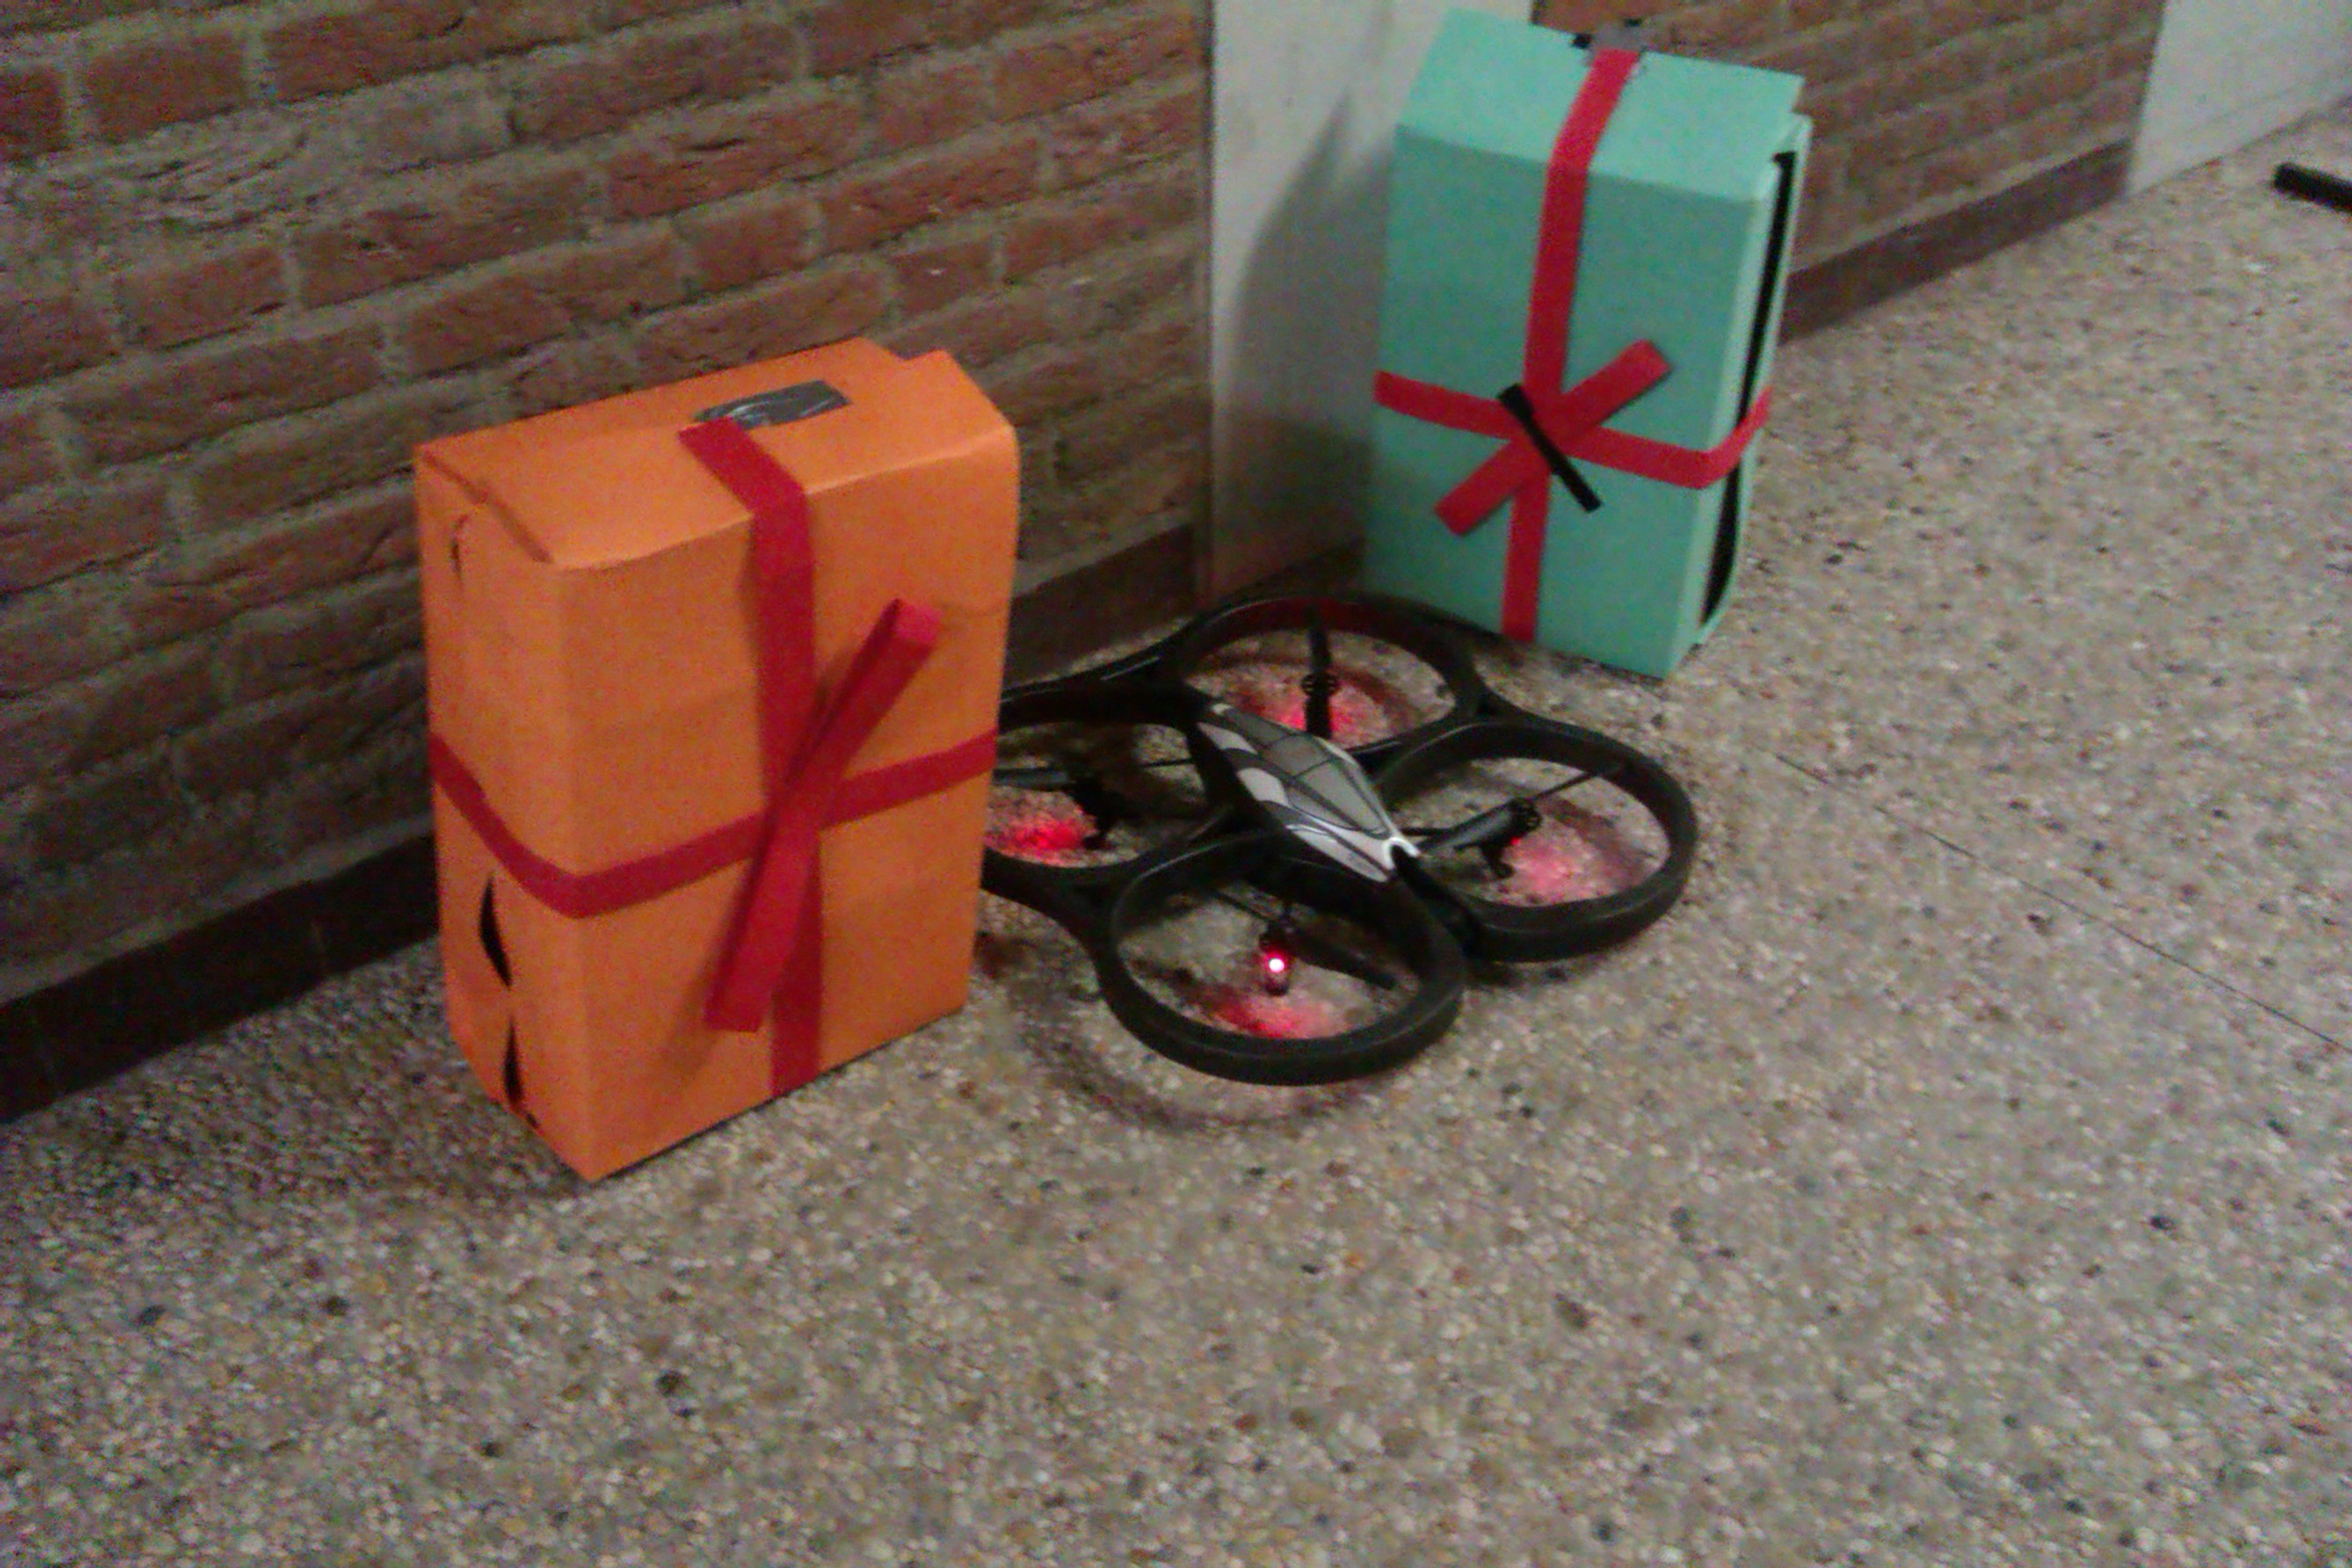
\includegraphics[width=0.5\textwidth]{images/presentsAndDrone}
\end{figure}
%%%%%%%%%%%%%%%%%%%%%%%%%%%%%%%%%%%%%%%%%%%%%%%%%%%%%%%%%%%%%%%%%%%%%%%%%%%%%%%
% BIBLIOGRAPHY
%%%%%%%%%%%%%%%%%%%%%%%%%%%%%%%%%%%%%%%%%%%%%%%%%%%%%%%%%%%%%%%%%%%%%%%%%%%%%%%
\bibliographystyle{plain}
\bibliography{bibliography}

\end{document}
